% ---
% Capitulo de revisão de literatura
% ---
\chapter{Padrões de Projeto}
% ---

Durante o processo de desenvolvimento de software 
orientado a objetos, 
problemas de design são comuns durante a 
fase de projeto. Alguns desses problemas 
eram tão comuns que foi feito um esforço para catalogá-los 
em um livro \cite{gamma:1995} que oferece possíveis soluções para os mesmos. 
Essas soluções tornaram-se conhecidas como 
os Padrões de Projeto Gang of Four, abreviados 
para Padrões de Projeto GoF.

Por definição, um padrão de projeto é uma solução 
reutilizável para um problema comum de design. Apesar 
deste trabalho se restringir ao contexto de engenharia 
de software, o conceito foi introduzido pelo arquiteto 
Christopher Alexander no livro A Pattern Language 
\cite{alexanderpatternlanguage}.

Com foco no design orientado a objetos, hoje os 
padrões GoF estão entre os padrões de 
projeto de software mais conhecidos. Os responsáveis 
por compilá-los foram Erich Gamma, Richard Helm, 
Ralph Johson e John Vlissides, o que deu origem ao 
nome Gang of Four. Ao todo, vinte e três 
padrões foram catalogados, os mesmos que serão o alvo 
deste trabalho.

De acordo com o livro, um padrão possui quatro elementos 
essenciais: um nome, um problema, uma solução e suas 
consequências. O nome é uma característica importante 
por tornar mais fácil referenciar um padrão. O problema 
descreve a situação em que o padrão é aplicado e 
a solução descreve como um conjunto de elementos pode 
resolver o problema proposto. Já as consequências 
mostram as vantagens e desvantagens do uso do padrão 
para um problema.

Como forma de organizar os padrões, o livro os separa 
por finalidade e por escopo. A separação por finalidade 
divide os padrões entre padrões criacionais, 
destinados ao processo de criação de objetos, padrões 
estruturais, que lidam com a forma em que o conjunto de 
classes e objetos está disposto e padrões comportamentais, 
focados na forma em que classes e objetos comunicam-se 
e distribuem suas responsabilidades. A separação por 
escopo divide os padrões no escopo de classe ou de objeto, 
onde o primeiro lida com a relação entre classes e 
subclasses através de herança, enquanto o segundo lida 
com formas de relacionamento mais dinâmicas entre os 
objetos, como delegação. Os padrões nesse trabalho 
serão separados apenas por finalidade, porém 
características que remetem ao escopo 
podem ser consideradas durante a análise.


\section{Exemplo de padrão de projeto: Singleton}

A descrição de cada padrão no livro segue uma estrutura 
muito similar, utilizada principalmente para apresentar 
os quatro elementos essenciais mencionados anteriormente. 
Como exemplo para demonstrar a forma como o livro 
apresenta cada padrão, o padrão criacional Singleton será 
demonstrado com uma breve explicação de cada tópico. 
Uma descrição mais sucinta dos outros padrões será 
apresentada durante o desenvolvimento deste 
trabalho, onde serão considerados apenas os elementos 
essenciais dos padrões na análise 
a partir do paradigma funcional.

\subsection*{Intenção}

A intenção é uma forma curta de descrever o que o padrão 
faz, qual é sua intenção e que problema ele busca resolver. 
O Singleton busca garantir que uma classe tenha apenas uma
instância, acessível globalmente.

\subsection*{Motivação}

Este tópico ilustra um problema e demonstra como a estrutura 
do padrão o soluciona, tornando mais simples a compreensão 
das descrições mais abstratas que vêm a seguir. Para o 
Singleton, é utilizado como exemplo o spooler de uma 
impressora, um sistema de arquivos ou um gerenciador de 
janelas. Para todos esses casos, apenas um objeto precisa existir, 
ou seja, uma classe que representa algum desses elementos 
só precisa possuir uma instância de fácil acesso. É proposto 
tornar a própria classe responsável por gerenciar essa 
instância, garantindo que nenhum outra instância dela 
mesma seja criada e garantindo um meio de acesso a essa 
única instância.

\subsection*{Aplicabilidade}

A aplicabilidade descreve situações nas quais o padrão 
pode ser aplicado, exemplos de maus projetos que ele pode 
ajudar a tratar e ainda como reconhecer essas situações. 
No caso do Singleton, ele é utilizável quando for necessário 
possuir apenas uma instância de uma classe através de um 
ponto de acesso conhecido e quando essa única instância 
precisa ser extensível através de subclasses. 

\subsection*{Estrutura}

A estrutura apresenta o padrão graficamente, através de uma 
notação baseada na Object Modeling Technique (OMT) e às vezes 
em diagramas de interação. No caso do Singleton, apenas o 
seguinte diagrama é utilizado:

\begin{figure}[htb]
	\caption{\label{fig_grafico}Estrutura do Singleton utilizada como exemplo}
	\begin{center}
	    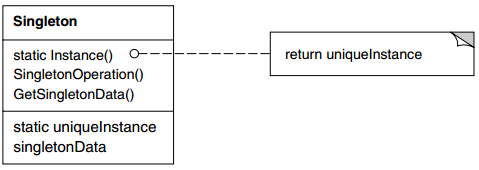
\includegraphics[scale=0.5]{4_referencial_teorico/2_padroes-projeto/singleton_structure.png}
    \end{center}
    \legend{Fonte: \cite{gamma:1995}}
\end{figure}

\subsection*{Participantes}

Descreve as responsabilidades de cada classe que 
participa do padrão. Neste caso, existe 
apenas uma: o próprio Singleton, que define 
a operação de classe Instance, permitindo aos clientes 
acessarem sua única instância. Também pode ser o 
responsável por criar sua própria instância única.

\subsection*{Colaborações}

Este tópico explica como as classes participantes 
colaboram para executar as responsabilidades 
especificadas. Para o Singleton, os clientes (ou seja, 
os objetos que o acessam) acessam a instância única 
pela operação Instance.

\subsection*{Consequências}

As consequências descrevem os custos e benefícios para 
que o padrão possa realizar seu objetivo, além dos 
aspectos da estrtura de um sistema que ele permite variar 
independentemente. O Singleton enumera cinco benefícios:

Primeiro, acesso controlado à instância única, já que 
a única instância é encapsulada dentro da classe 
Singleton, ela possui controle total de como e quando 
ela pode ser acessada pelos clientes.

Segundo, espaço de nomes reduzido. Uma alternativa 
para o Singleton talvez fosse o uso de variáveis 
globais, porém o padrão evita que o espaço de nomes 
seja poluído com variáveis globais que utilizam 
instâncias únicas.

Terceiro, ele permite um refinamento de operações e da 
representação, ou seja, permite ao Singleton ter 
subclasses.

Quarto, permite um número variável de instâncias. Nesse 
caso, o padrão permite que, após ele ser implementado, 
seja simples mudar de ideia e a própria classe Singleton, 
dentro da operação Instance, volte a permitir um número 
indefinido ou até controlado de instâncias.

Quinto, é mais flexível do que operações de classe. Além 
das variáveis globais, operações de classe seriam outra 
alternativa para o Singleton, porém isso tornaria mais 
difícil voltar a ter mais de uma instância da classe, 
além de impedir, em certas linguagens, que subclasses 
redefinam operações estáticas polimorficamente.

\subsection*{Implementação}

Explicita sugestões, técnicas ou riscos que devem 
ser conhecidos durante a implementação do padrão, 
além de considerações específicas de algumas 
linguagens. Para o Singleton, existem duas 
explicações de implementação.

A primeira refere-se à garantia da existência de 
apenas uma instância, onde é sugerido tornar a operação 
de criação do Singleton em uma operação de classe 
que possui acesso a um atributo que armazena a 
instância do Singleton, caso já exista. A segunda 
trata da criação de subclasses da classe Singleton, 
onde é sugerido registrar cada instância por nome 
para que uma classe cliente possa acessar o singleton 
desejado sem precisar conhecer todas as instâncias 
existentes. Ambas as implementações são 
exemplificadas na seção de exemplo de código.


\subsection*{Exemplo de Código}

Como o nome já diz, demonstra o padrão através de 
um exemplo em código. O exemplo do Singleton é um 
construtor de labirintos, onde a classe que é 
responsável pela fabricação dos labirintos necessita 
de apenas uma instância. O código \ref{singletonnosub}
apresenta a implementação do padrão sem o uso de 
subclasses, enquanto o código \ref{singletonsub} 
apresenta uma versão com o uso de subclasses, 
onde as subclasses referenciadas são BombedMazeFactory  
e EnchantedMazeFactory. 
Ambos estão na linguagem C++ e foram retirados 
do livro, porém a implementação pode ser feita 
de forma equivalente em qualquer linguagem 
orientada a objetos.

\begin{lstlisting}[caption={Exemplo de Singleton sem subclasses}, label=singletonnosub]
    
    class MazeFactory {
    public:
        static MazeFactory* Instance();

        // interface existente vai aqui
    protected:
        MazeFactory();
    private:
        static MazeFactory* _instance;
    };


    // implementação:

    MazeFactory* MazeFactory::_instance = 0;

    MazeFactory* MazeFactory::Instance () {
        if (_instance == 0) {
            _instance = new MazeFactory;
        } 
        return _instance;
    } 

\end{lstlisting}
\legend{Fonte: \cite{gamma:1995}}


\begin{lstlisting}[caption={Exemplo de Singleton com subclasses},label=singletonsub]
    
    MazeFactory* MazeFactory::Instance () {
        if (_instance == 0) {
            const char* mazeStyle = getenv("MAZESTYLE");

            if (strcmp(mazeStyle, "bombed") == 0) {
                _instance = new BombedMazeFactory;

            } else if (strcmp(mazeStyle, "enchanted") == 0) {
                _instance = new EnchantedMazeFactory;

            // ... outras subclasses possíveis

            } else { // default
                _instance = new MazeFactory;
            }
        }
        return _instance;
    } 

\end{lstlisting}
\legend{Fonte: \cite{gamma:1995}}


\subsection*{Usos Conhecidos}

Demonstra usos desse padrão em sistemas reais. No caso 
do Singleton, é mencionado o relacionamento entre 
classes e suas metaclasses. Um exemplo atual de uso 
de Singleton é a ferramenta de injeção de dependência 
do .NET Core, onde um serviço 
pode comportar-se como um Singleton\cite{didotnet}.

\subsection*{Padrões Relacionados}

Os padrões relacionados apresentam padrões que 
possuem alguma relação ou que podem ser usados juntos 
do padrão proposto. São mencionados padrões que 
podem ser implementados utilizando o Singleton, que 
são o AbstractFactory, o Builder e o Prototype.

